\subsection{Random Access Memory}

\subsubsection{RAM access time}
\paragraph{Methodology}
We measured the back-to-back-load RAM access latency, because it is well accepted by most software developers and system researchers. The way we measure the RAM access latency is making the program iterating a array of specific size for bunch of times and averaging it to eliminate the noise. The size of the array we used are larger than 256KB, which is larger than the total amount of L1 cache and L2 cache. We did multiple number of tests on iterating the first k element of the array, so that certain part of the data will be cached into L1 cache or L2 cache.
We expected to see the RAM access time increases as it goes from L1, L2 to main memory. Basically saying there would be a significant difference among the following three cases: 
1. iteration of the first 32KB data or less (fit into L1 cache)
2. iteration of the first 288KB data or less (fit into L1+L2 cache)
3. iteration of all the whole array(doesn’t fit into caches).
\paragraph{Predictions}
\paragraph{Results}
We are going to present the result table for stride 11 and the plotted graph for different strides from 1 to 15.
\begin{center}
\begin{tabular}{| r | l | l | l | r |}
\hline
Size of array 	& Hardware cost 	& Software cost 	& Prediction 	& Measured \\ \hline
512B 			&				&				&			&3.895 cycles	\\ \hline
1KB 			&				&				&			&3.886 cycles		\\ \hline
2KB 			&				&				&			&3.885 cycles		\\ \hline
4KB 			&				&				&			&3.886 cycles		\\ \hline
8KB 			&				&				&			&3.886 cycles		\\ \hline
16KB 			&				&				&			&3.888 cycles		\\ \hline
32KB 			&				&				&			&3.891 cycles		\\ \hline
64KB 			&				&				&			&5.949 cycles		\\ \hline
128KB 		&				&				&			&5.945 cycles		\\ \hline
256KB 		&				&				&			&6.209 cycles		\\ \hline
512KB 		&				&				&			&10.314 cycles		\\ \hline
1MB 			&				&				&			&10.399 cycles		\\ \hline
2MB 			&				&				&			&10.757 cycles		\\ \hline
4MB 			&				&				&			&15.585 cycles		\\ \hline
8MB 			&				&				&			&30.265 cycles		\\ \hline
16MB 			&				&				&			&37.458 cycles		\\ \hline
32MB 			&				&				&			&37.686 cycles		\\ \hline
64MB 			&				&				&			&37.092 cycles		\\ \hline
128MB 		&				&				&			&37.619 cycles		\\ \hline

\hline
\end{tabular}
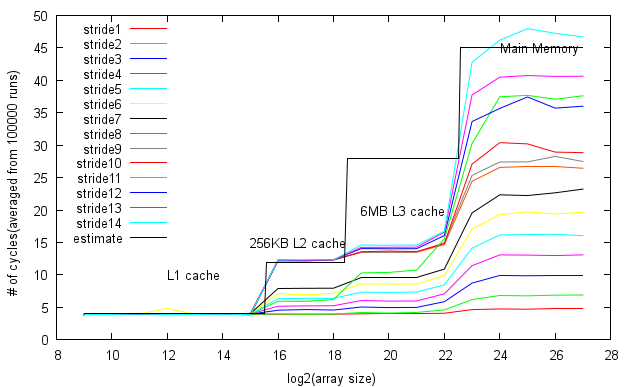
\includegraphics[scale=0.8]{memoryLatencyImage}
\end{center}

\paragraph{Accuracy of Estimates}
\paragraph{Success of Methodology}

The result we got from our measurement shown that //TODO actual result






\subsubsection{RAM bandwidth}
\paragraph{Methodology}

We used an array with size 16MB, so that it is larger than the cache size (6MB including fancy L3 cache). At the same time, it still fits into the main memory. We iterated through the list and do both read and write. We did read by just doing a[i]+0 and write by doing a[i] = a[i]+1. We would expect read is faster than write operation, because the system need to make sure the data is actually write to the memory after performed the write operation. While there is no such issue for read operation.
\paragraph{Predictions}
\paragraph{Results}

\begin{center}
\begin{tabular}{| l | l | l | l | l |}
\hline
Operation & Hardware cose & Software cost & Prediction & Measured \\
\hline
\end{tabular}
\end{center}

\paragraph{Accuracy of Estimates}
\paragraph{Success of Methodology}





\subsubsection{Page fault service time}
\paragraph{Methodology}
In order to manually create a page fault situation, we used two really large array which as the same size as main memory. Then we are going to iterate through the first array, basically means put it into main memory first. Afterwards, we iterate through the second array so that the first array will be totally paged out to hardddisk after that. The page fault service time is going to be the time it takes for us to get the value of element from first array at this point.This forces the page to swap gives us the right page fault service time. 
\paragraph{Predictions}
\paragraph{Results}

\begin{center}
\begin{tabular}{| l | l | l | l | l |}
\hline
Operation & Hardware cose & Software cost & Prediction & Measured \\
\hline
\end{tabular}
\end{center}

\paragraph{Accuracy of Estimates}
\paragraph{Success of Methodology}
